%%%%%%%%%%%%%%%%%%%%%%%%%%%%%%%%%%%%%%%%%%%%%%%%%%%%%%%%%%%
% --------------------------------------------------------
% Tau
% LaTeX Template
% Version 2.4.4 (28/02/2025)
%
% Author: 
% Guillermo Jimenez (memo.notess1@gmail.com)
% 
% License:
% Creative Commons CC BY 4.0
% --------------------------------------------------------
%%%%%%%%%%%%%%%%%%%%%%%%%%%%%%%%%%%%%%%%%%%%%%%%%%%%%%%%%%%

\documentclass[9pt,a4paper,twocolumn,twoside]{tau-class/tau}
\usepackage[brazil]{babel}

\usepackage{booktabs}
\usepackage{float}
\usepackage{graphicx}
\usepackage{siunitx}
\usepackage{tikz}
\usetikzlibrary{arrows.meta, positioning}

%% Spanish babel recomendation
% \usepackage[spanish,es-nodecimaldot,es-noindentfirst]{babel} 

%% Draft watermark
% \usepackage{draftwatermark}

%----------------------------------------------------------
% TITLE
%----------------------------------------------------------

\journalname{Relatório de Sistemas de Controle I - Etapa 3}
\title{Controle de Estabilização de um Pêndulo Invertido Rotacional}

%----------------------------------------------------------
% AUTHORS, AFFILIATIONS AND PROFESSOR
%----------------------------------------------------------

\author[a,1]{JOSÉ A. DA SILVA}
\author[b,2]{KAUA LESSA L. DOS SANTOS }
\author[c,3]{PABLO MUNIH S. DE CARVALHO}
\author[d,4]{PLÁCIDO AUGUSTUS DE O. CORDEIRO}

%----------------------------------------------------------

\affil[a]{Engenharia da Computação, Universidade Federal de Alagoas}
\affil[b]{Engenharia da Computação, Universidade Federal de Alagoas}
\affil[c]{Engenharia da Computação, Universidade Federal de Alagoas}

\professor{Prof. ICARO BEZERRA QUEIROZ DE ARAUJO}

%----------------------------------------------------------
% FOOTER INFORMATION
%----------------------------------------------------------

\institution{Universidade Federal de Alagoas}
%\footinfo{\LaTeX\ Template}%
\theday{\today}
% \leadauthor{Aluno et al.} %
\course{Engenharia da Computação}

%----------------------------------------------------------
% ABSTRACT AND KEYWORDS
%----------------------------------------------------------

\begin{abstract}    
    Esta etapa final do projeto engloba a montagem experimental do protótipo e o projeto do controlador para o pêndulo invertido rotacional.
    Inicialmente, o modelo matemático derivado e simulado nas etapas anteriores é submetido a um processo de validação, comparando-se suas
    respostas com dados experimentais coletados do sistema físico montado. Em seguida, procede-se ao projeto de um controlador em malha
    fechada, com base em técnicas de análise e síntese de sistemas de controle, com o objetivo de estabilizar o pêndulo na posição
    vertical invertida. O controlador projetado é então implementado e testado, tanto em simulação quanto no protótipo real,
    permitindo uma análise crítica do desempenho do sistema controlado e da fidedignidade do modelo matemático adotado. 
\end{abstract}


%----------------------------------------------------------

\keywords{pêndulo invertido, controle rotacional, estabilização, sistemas não lineares}

%----------------------------------------------------------

\begin{document}
		
    \maketitle 
    \thispagestyle{firststyle} 
    \tauabstract 
    % \tableofcontents
    % \linenumbers 
    
%----------------------------------------------------------

\section{Introdução}
    \taustart{A} etapa anterior focou na modelagem e simulação do sistema. A descrição da dinâmica do sistema foi realizada 
    utilizando a equação de Euler-Lagrange, resultando em equações diferenciais ordinárias não lineares que descrevem o
    comportamento do braço e do pêndulo. Foi realizada a linearização em torno de (\(\alpha = 0\)), o que permitiu a
    obtenção de uma representação em espaço de estados e da respectiva função de transferência \(G(s) = \frac{\alpha(s)}{V_m(s)}\),
    que relaciona a tensão aplicada ao motor com o ângulo do pêndulo. Em seguida, a função de transferência obtida foi
    analizada, assim como a resposta do sistema em malha aberta, o que revelou um sistema intrinsecamente instável. Esta seção do 
    relatório busca recapitular a etapa anterior e definir os objetivos desta etapa final do projeto. 

    \subsection{Modelagem Matemática}
    
    A modelagem apresentada na etapa anterior segue de perto a apresentada em \cite{ramos2011rotary}, que descrevem detalhadamente o
    procedimento de modelagem do pêndulo invertido rotacional (Pêndulo de Furuta). Inicialmente, foi estabelecida a convenção de coordenadas
    ilustrada na figura \ref{fig:angulo_pendulo}, onde o ângulo de rotação do braço horizontal é denotado por \(\theta\) e o ângulo do pêndulo com o plano vertical é
    definido como \(\alpha\). O estado de interesse corresponde explicitamente a \(\alpha = 0\), onde o pêndulo se encontra na vertical.

    \subsubsection*{Lagrangiana e Equação de Euler-Lagrange}
    Ao estabelecer a convenção de coordenadas, é possível encontrar as energias potenciais e cinéticas do sistema, assim é permitindo 
    expressar a Lagrangiana da seguinte forma:

    \begin{equation}
    \mathcal{L} = \tfrac{1}{2}(J_{eq} + m r^2)\dot{\theta}^2
        - m L r \cos(\alpha)\,\dot{\theta}\dot{\alpha}
        + \tfrac{2}{3} m L^2 \dot{\alpha}^2
        - m g L \cos(\alpha)
    \end{equation}

    Onde $J_{eq}$ é o momento de inércia equivalente à carga do motor, $m$ é a massa do braço horizontal, $r$ é o comprimento do braço
    rotativo, $L$ é a distância até o centro de massa do pêndulo e $g$ é a aceleração da gravidade.
    
    No sistema é possível identificar
    duas coordenadas generalizadas: \(\theta\) e \(\alpha\). Dessa forma, aplicando a equação de Euler-Lagrange as coordenadas generalizadas
    e linearizando em torno de $\alpha \approx 0$, obtemos as seguintes equações: \\

    \begin{align}
    (J_{eq} + m r^2)\ddot{\theta} - m L r \ddot{\alpha} &= T_{output} - B_{eq}\dot{\theta} 
    && \text{(Braço)} \\
    \tfrac{4}{3} m L^2 \ddot{\alpha} - m L r \ddot{\theta} - m g L \alpha &= 0
    && \text{(Pêndulo)}
    \end{align}

    \begin{figure}[H]
    \centering
    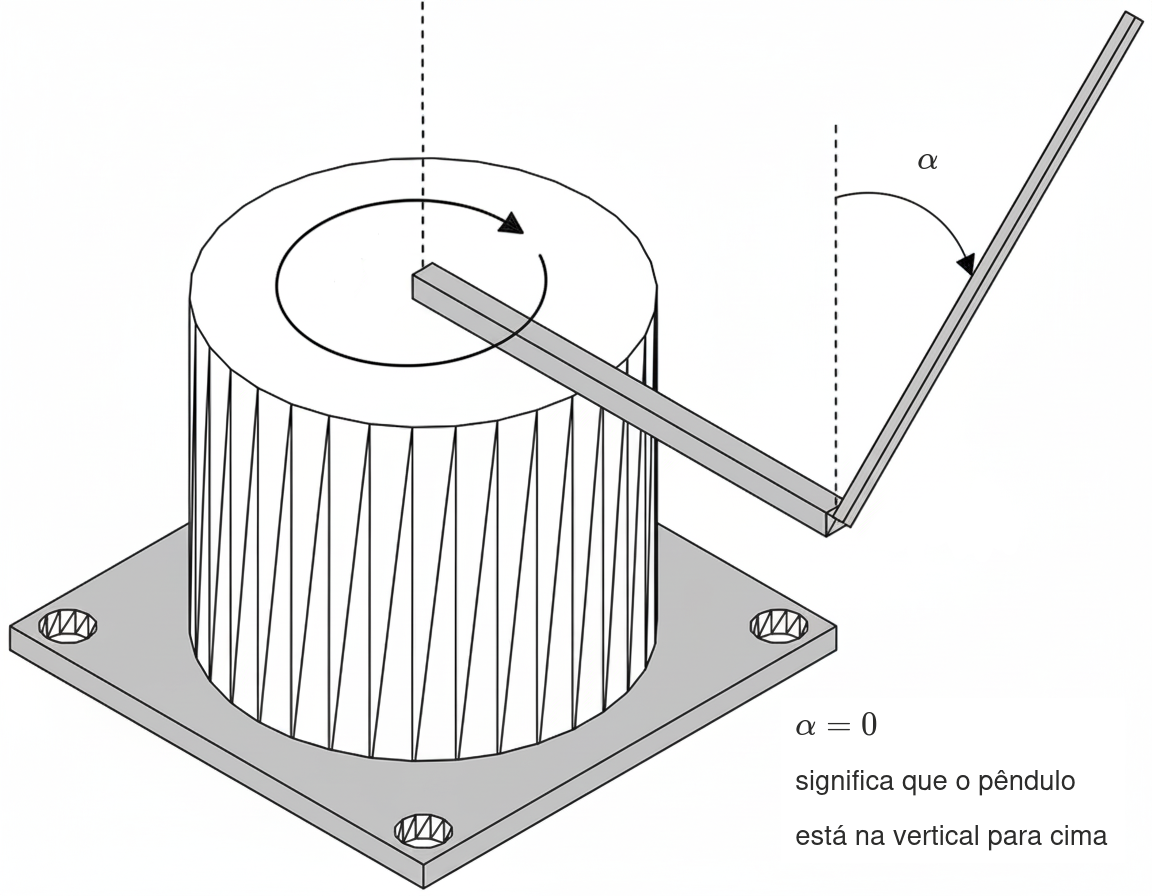
\includegraphics[width=0.9\columnwidth]{figures/angulo_pendulo.png} % Ajustado para columnwidth
    \caption{Definição das variáveis angulares do Pêndulo de Furuta, com o ângulo do braço \(\theta\) e o ângulo do pêndulo \(\alpha\). A posição de equilíbrio instável (\(\alpha=0\)) é indicada.}
    \label{fig:angulo_pendulo}
    \end{figure}

    \subsubsection*{Representação em Espaços de Estados e Função de Transferência}
    O torque de saída do motor aplicado ao sistema é dado por:

    \begin{equation}
    T_{output} = \frac{\eta_m \eta_g K_t K_g}{R_m} \left( V_m - K_G K_m \dot{\theta} \right) 
    \label{eq:torque}
    \end{equation}

    Combinando as equações de movimento obtidas, a representação em espaço de estados pode ser escrita como:

    \begin{equation}
\begin{bmatrix}
\dot{\theta} \\
\dot{\alpha} \\
\ddot{\theta} \\
\ddot{\alpha}
\end{bmatrix}
=
\begin{bmatrix}
0 & 0 & 1 & 0 \\
0 & 0 & 0 & 1 \\
0 & 39.32 & -14.52 & 0 \\
0 & 81.78 & -13.98 & 0
\end{bmatrix}
\begin{bmatrix}
\theta \\ \alpha \\ \dot{\theta} \\ \dot{\alpha}
\end{bmatrix}
+
\begin{bmatrix}
0 \\ 0 \\ 25.54 \\ 24.59
\end{bmatrix} V_m
\label{eq:estadoNum}
\end{equation}

\begin{equation}
Y =
\begin{bmatrix}
1 & 0 & 0 & 0 \\
0 & 1 & 0 & 0
\end{bmatrix}
\begin{bmatrix}
\theta \\ \alpha \\ 
\end{bmatrix}
+
\begin{bmatrix}
0 \\ 0
\end{bmatrix} V_m
\end{equation}

\subsection{Obtenção da Função de Transferência}
A partir do modelo em espaço de estados (Eq.~\ref{eq:estadoNum}), pode-se obter a 
função de transferência que relaciona a entrada do sistema (tensão no motor $V_m$) 
com a saída escolhida (ângulo do pêndulo $\alpha$). Para isso, foi utilizada a 
função \texttt{tf()} do \textit{MATLAB}, que converte a representação em espaço 
de estados para a forma de função de transferência. Dessa forma, obtemos a relação
\(G(s) = \frac{\alpha(s)}{V_m(s)}\) a seguir: \\

\begin{equation}
    G(s) = \frac{\alpha(s)}{V_m(s)}
         = \frac{24.59\,s - 0.0024}{s^3 + 14.52\,s^2 - 81.78\,s - 637.8}
\end{equation}

\subsection{Análise do Modelo}
Após a obtenção da função de transferência que descreve a dinâmica entre a tensão aplicada ao motor e o ângulo do pêndulo, procede-se
à análise matemática do sistema em malha aberta. Embora ainda não haja controle implementado, esta etapa é essencial para compreender
as limitações naturais do sistema e justificar a necessidade de técnicas de estabilização.

\subsubsection*{Ordem e grau relativo}
\begin{itemize}
    \item \textbf{Ordem do sistema:} 3 (denominador de grau 3) — sistema de 3ª ordem.
    \item \textbf{Grau do numerador:} 1.
\end{itemize}

\subsubsection*{Polos e estabilidade}
As raízes do denominador (polos) obtidos numericamente são aproximadamente:
\[
p_1 \approx -17.12,\qquad p_2 \approx -4.94,\qquad p_3 \approx +7.54.
\]
Como existe um polo em \(\,p_3 \approx +7.54\) (semiplano direito), o sistema é \textbf{instável em malha aberta}. A raiz do numerador
(zero) é aproximadamente:
\[
z \approx +9.76\times 10^{-5}.
\]

O sistema possui, portanto, um zero no semiplano direito (RHP), caracterizando-o como \textbf{não mínimo-fase}, a principal consequência
disso é a tendência do sistema de apresentar uma resposta inversa (\textit{undershoot}).

\subsubsection*{Ganho DC}
O ganho estático do sistema é: \[G(0)=\frac{-0.0024}{-637.752}\approx 3.76\times 10^{-6}.\] O valor é muito pequeno, mas na prática
a dinâmica é dominada pelo polo instável.

\subsubsection*{Tipo do sistema}
Não há polos em $s=0$, logo o sistema é do \textbf{tipo 0}. Em teoria isso significa erro finito para entrada em degrau,
mas devido à instabilidade, em malha aberta a saída tende a divergir.

\subsection{Simulação Computacional}
Para validar e visualizar o comportamento dinâmico previsto pela análise matemática, o sistema foi simulado no ambiente
\textit{MATLAB/Simulink}. Utilizando a função de transferência \(G(s)\) obtida, foram analisadas as respostas do sistema
em malha aberta a três sinais de entrada canônicos: impulso, degrau e rampa.

\begin{figure}[H]
    \centering
    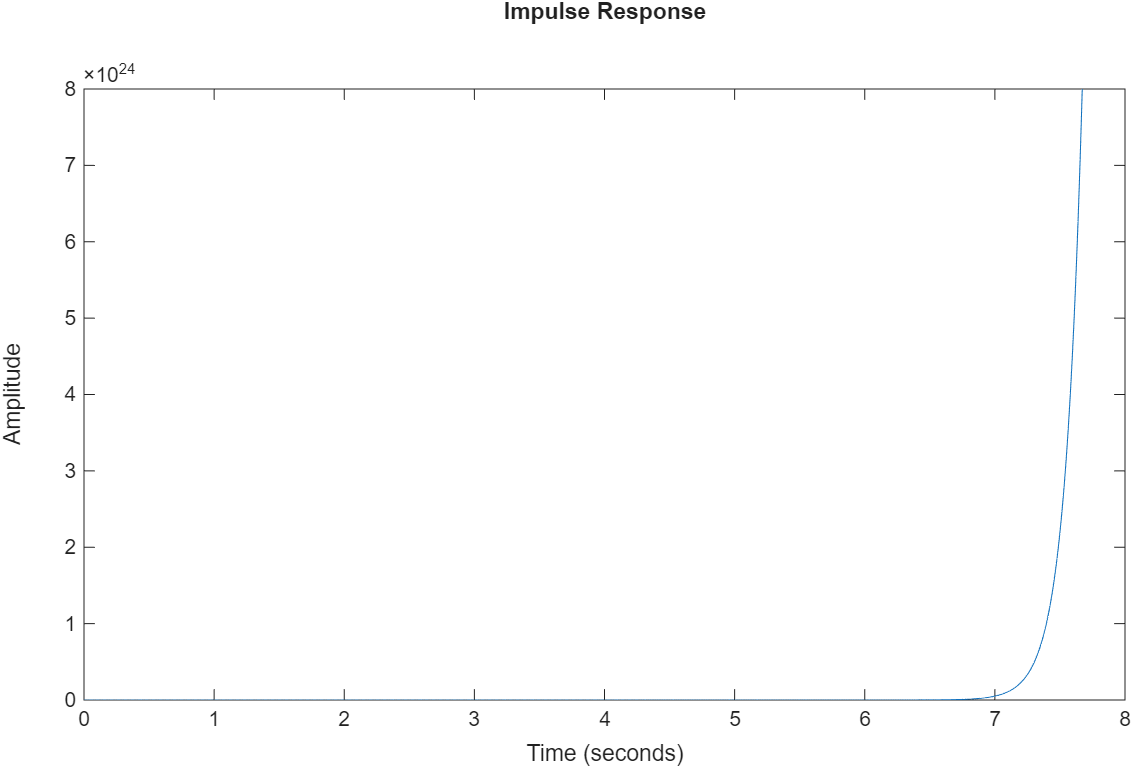
\includegraphics[width=0.45\textwidth]{figures/impulse_response.png}
    \caption{Resposta ao impulso do sistema em malha aberta.}
    \label{fig:impulse}
\end{figure}

\begin{figure}[H]
    \centering
    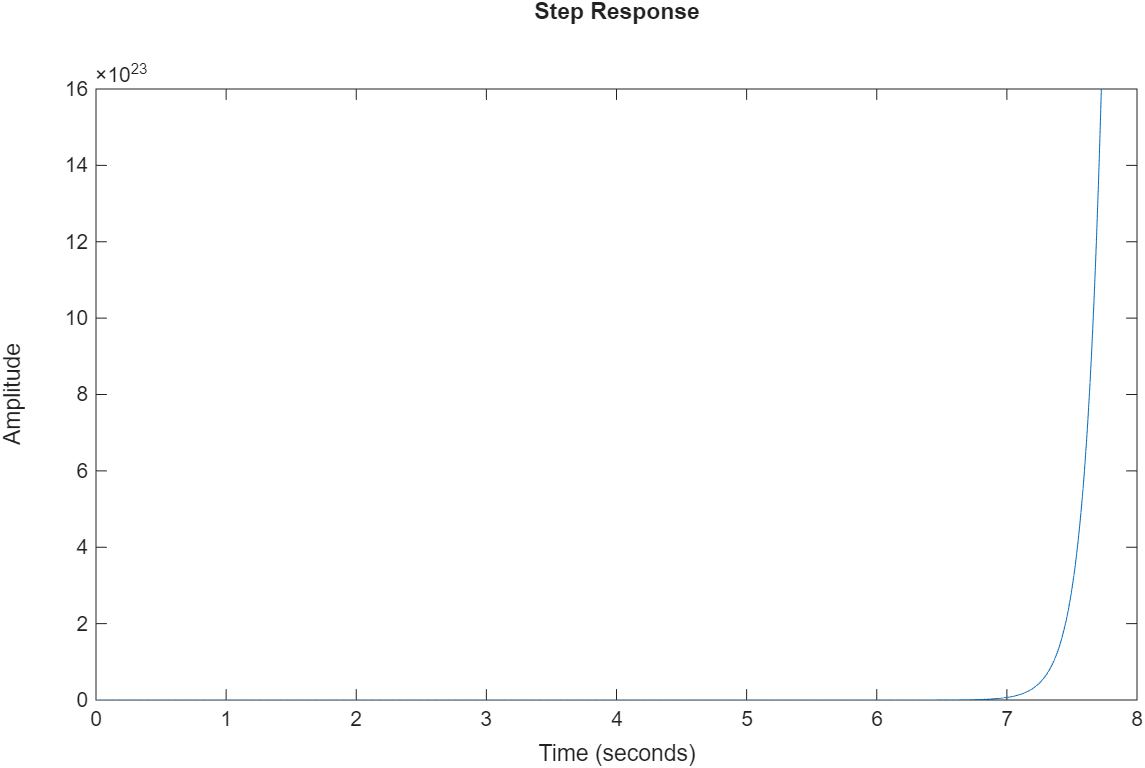
\includegraphics[width=0.45\textwidth]{figures/step_response.png}
    \caption{Resposta ao degrau do sistema em malha aberta.}
    \label{fig:step}
\end{figure}

\begin{figure}[H]
    \centering
    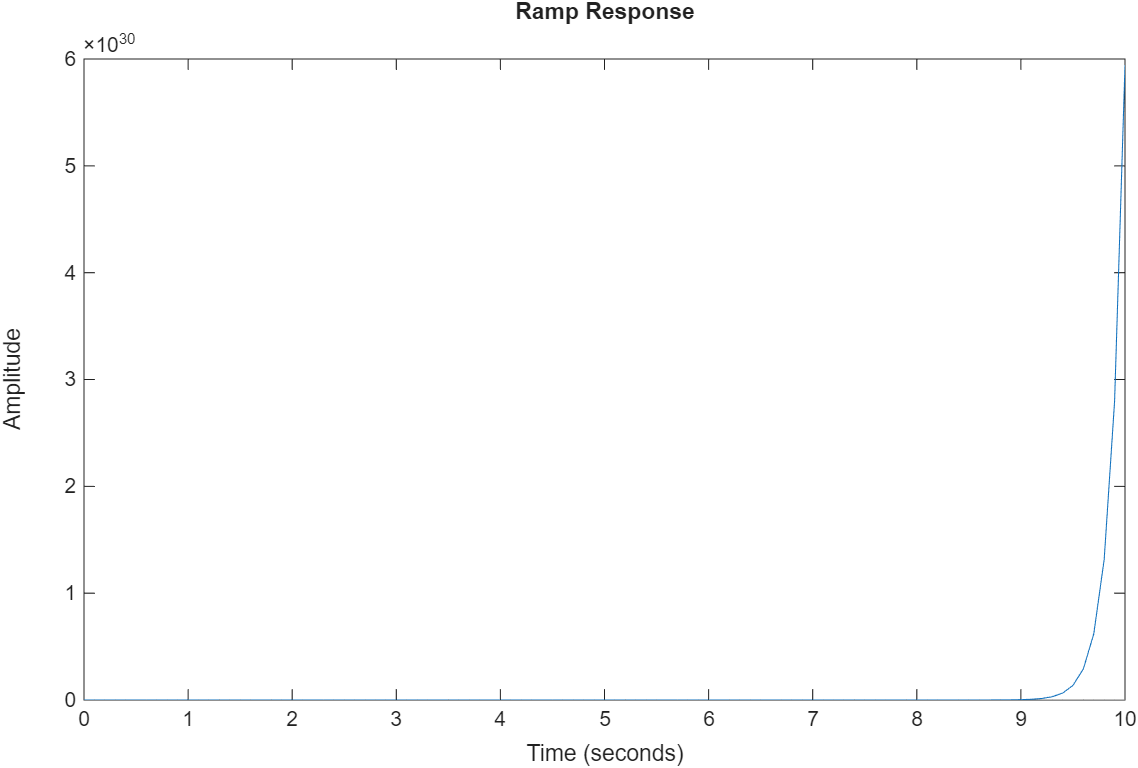
\includegraphics[width=0.45\textwidth]{figures/ramp_response.png}
    \caption{Resposta à rampa do sistema em malha aberta.}
    \label{fig:ramp}
\end{figure}

As simulações computacionais do sistema em malha aberta para entradas de impulso, degrau e rampa confirmaram visualmente a
instabilidade prevista pela análise teórica, com a saída divergindo exponencialmente em todos os cenários.

\subsection{Objetivos}
As simulações computacionais, assim como a análise do modelo em malha aberta, confirmaram a instabilidade intrínseca do sistema
físico e forneceram uma base sólida e indispensável para a fase do final do projeto. Esta última etapa consolida a
montagem prática e o controle do sistema, visando validar o modelo matemático e implementar uma estratégia de controle em malha
fechada. Os objetivos específicos incluem: (i) montar o protótipo físico e coletar dados experimentais para validação do modelo
teórico; (ii) comparar qualitativa e quantitativamente as respostas real e simulada, analisando eventuais discrepâncias;
(iii) projetar um controlador PID que atenda a requisitos de desempenho pré-definidos; (iv) implementar e testar o controlador
no protótipo real; e (v) avaliar criticamente o desempenho do sistema controlado, comparando os resultados práticos com as simulações.

\printbibliography

%----------------------------------------------------------

\end{document}